\section{Overview}
In this chapter is explained how the platform that has been described will be implemented and tested. The aim of testing is to find the majority of the the bugs in the code that the working team has been generated.
Moreover a detailed description of how components inside the code are integrated will be provided (chapter 5.3).While instead in chapter 5.2 there it's presented a description of which are the most important implementation strategy used for making the project.


\section{Implementation Plan}
The aim of this section is to describe the implementation strategies that will be used to implement, integrate and test the different components. The intention is to combine the pros of the bottom-up and threads strategies.

Using a thread strategy is functional because you can make progresses visible for users and other stakeholders.it's possible to use less drivers than expected but the integration progress is more complex.

The Top-down methodology will be used this way a basic sketch will be designed and then more complex functionalities will be added as thread unit when they are validated.

This implementation strategy allows different teams to work in parallel by accomplishing different task on their own and then every unit that has been validated will be added to the whole software architecture.
\pagebreak


\subsection{Features identification}
The features to implement are described starting from the requirements.
Some requirements need the implementation of new components while instead others require only some small changes.
Here a small recap of the most important ones.

\begin{enumerate}[label={[\textbf{F\arabic*}]}]

\item \textbf{Sign-in and sign-up}

This two features are really simple to test and the test methodology is equal for both operations it's important to distinguish the two figure of educator and student because they have different privileges and different types of interaction.
\item \textbf{Creation of a Tournament and a Battle}

This feature is a core feature which has to be tested right after the sign-up and sign-in feature.
it enables the educator to create a tournament and a battle therefore it enables the other characteristics that is possible to use inside the battle.

\item \textbf{Team Creation}:

this functionality gives the possibility to a student to create its own team and this gives also the possibility to a student to enroll in a tournament and on the other hand to be able to unlock some other features such as  upload the team code and so on.

\item \textbf{Battle Management}

For what concerns the battle management this feature groups a lot of functionalities such as verifying if the battle is ended eventually additional evaluation are needed and a notification is sent when the battle has ended so the core functionalities need to be tested as specified in previous part

\item  \textbf{Code evaluation}

The code evaluation is a feature in which the system send the code uploaded by the students to the appropriate tools and this component send the score to the platform. 

\item \textbf{Tournament Consolidation}

The tournament consolidation is a feature that enables the educator to close the tournament and in the meanwhile after the end of the tournament a notification in send to students involved in the tournament
\item \textbf{Badge Creation and assignment}

This functionality is the embodiment of the system gamification so it is a core characteristic of the system. Moreover it involves both user kind of users the educator who creates a badge and the student who has it assigned. So it is compulsory to test it

\end{enumerate} 
\pagebreak
The majority the features that are listed require the interaction  between application between client and server of the application.
So the dispatcher has to be developed at the very beginning,



\section{Component Integration and Testing}
In this section it is detailed which component is implemented in every stage of the development process and how the different components are implemented and tested

\begin{enumerate}[label={[\textbf{F\arabic*}]}]

\begin{figure}[!h]
    \item \textbf{Sign-in and sign-up}

    The only part that need to be tested is the interaction of the system with the interface with github because the authentication API provided is considered reliable by definition.  
        \centering
        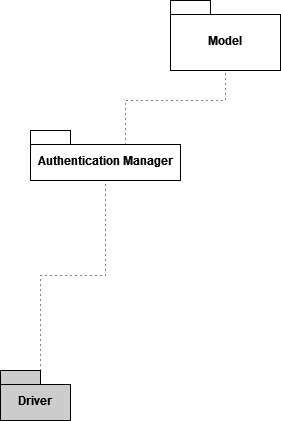
\includegraphics[width=6cm]{Images/testing.drawio(1).png}
        \caption{Sign in and Sign up developing}
        \label{fig: Sign in and Sign up developing}
       
    \end{figure}







\begin{figure}[!h]
\item \textbf{Creation of a Tournament and a Battle}

Here are added new features concerning the battles and the tournaments creation so new components and mangers need to be tested.


        \centering
        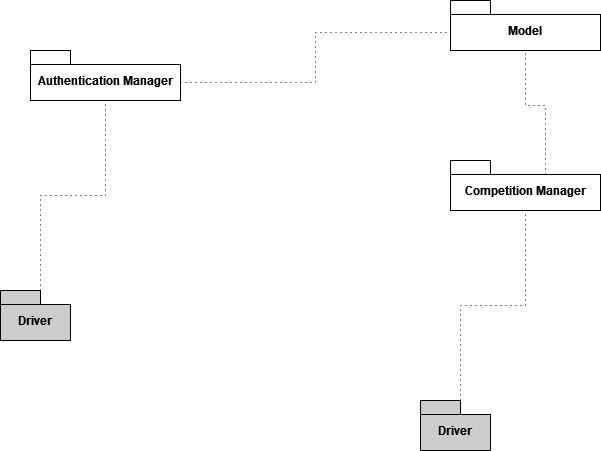
\includegraphics[width=12cm]{Images/Auth+comp.drawio.png}
        \caption{Creation of a Tournament and a Battle}
        \label{fig:Creation of a Tournament and a Battle}
       
    \end{figure}








\begin{figure}[!h]
\item \textbf{Team Creation}

Here it is explained how a team of student is created and for doing this some components are added to the previous diagram.


        \centering
        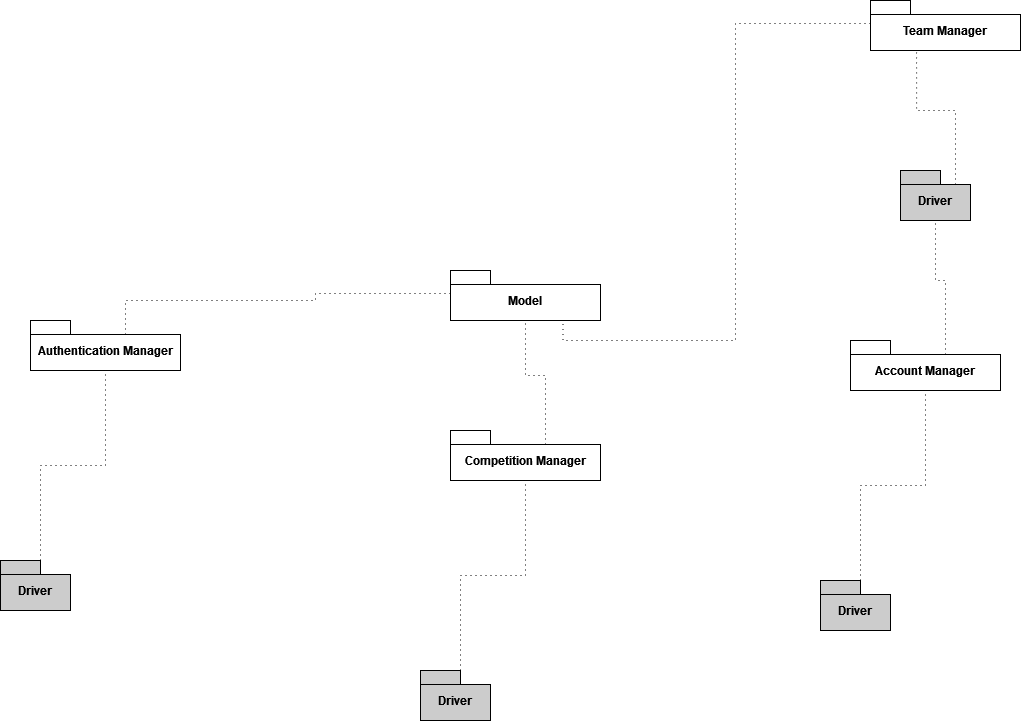
\includegraphics[width=12cm]{Images/Testing_Team_Creation.drawio.png}
        \caption{Team Creation}
        \label{fig:Team Creation}
       
    \end{figure}    

\begin{figure}[!h]
\item \textbf{Battle Management}

The battle management is managed by the Competition Manager that has been tested in a previous Diagram.The new component that has been tested is the Notification Manager important for sending notification to the different users.
         
    \centering
    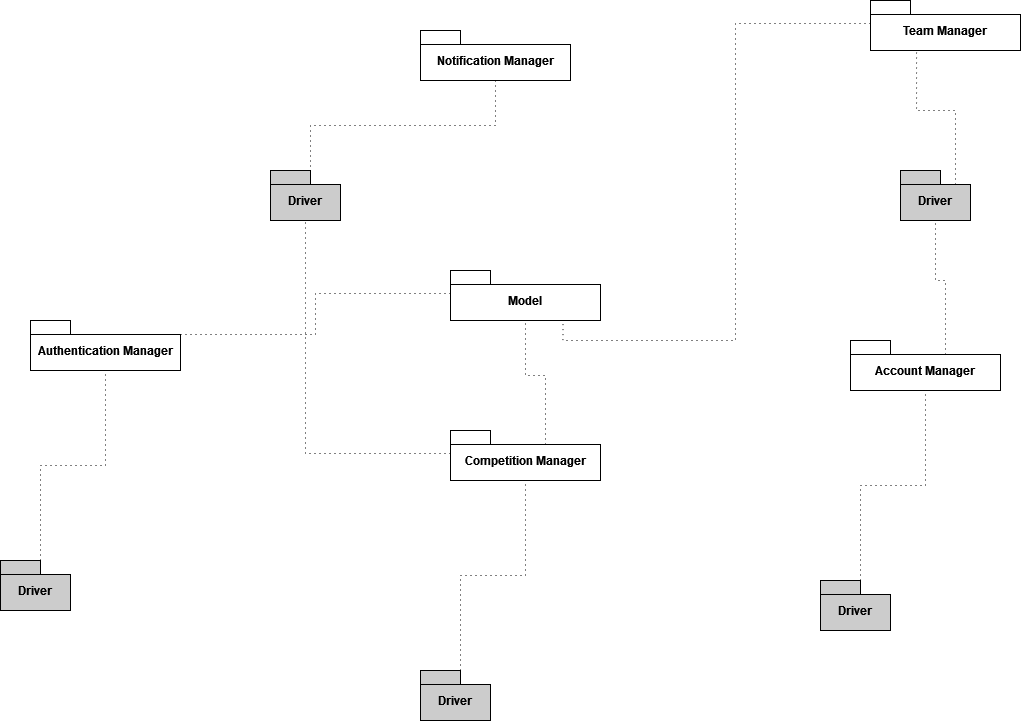
\includegraphics[width=11cm]{Images/TestingBattleManagement.drawio(2).png}
    \caption{Battle Management}
    \label{fig:Battle Management}
\end{figure}




\begin{figure}[!h]
\item \textbf{Code Evaluation}

Since the approach that has been used is the bottom-up with the combination of thread strategy the components has been added incrementally. The last component that has to be tested is the Competition Evaluation Manager which is necessary for the whole process of code evaluation and scoring but also for the submission of the codes and badge assignment.
         
    \centering
    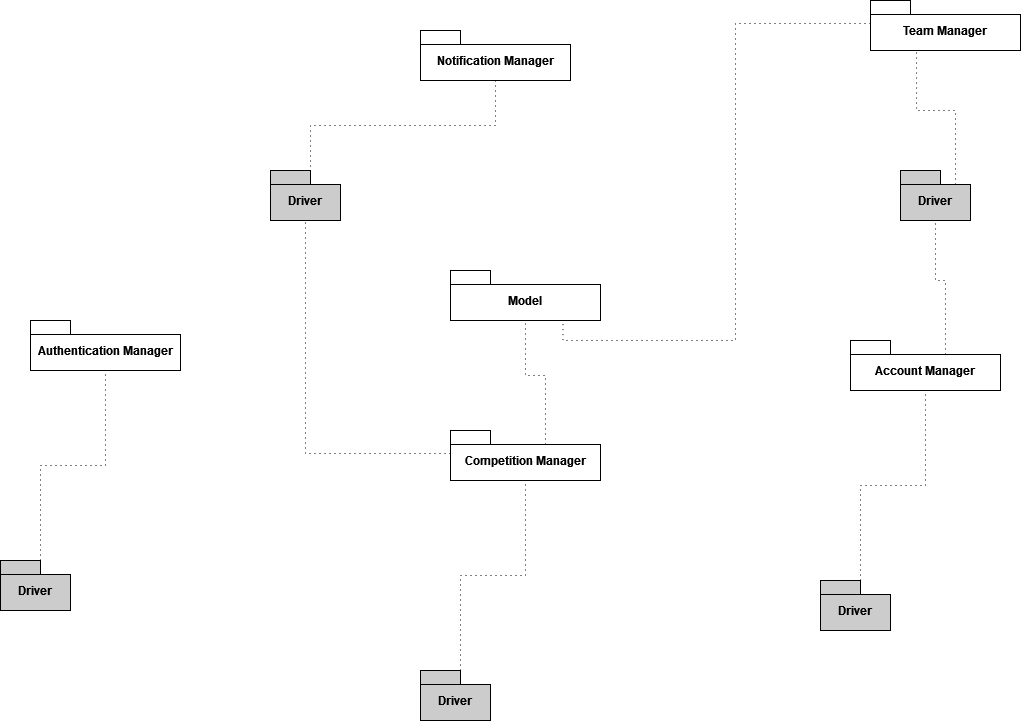
\includegraphics[width=11cm]{Images/TestingBattleManagement.drawio(1).png}
    \caption{Code Evaluation}
    \label{fig:Code Evaluation}
\end{figure}


\newpage
\item \textbf{Tournament Consolidation}

For what concerns this feature all the component has been tested in the previous diagrams.The only thing that to be tested is the piece of code in the Competition Manager that is in charge of consolidating the tournament. 

\item \textbf{Badge Creation and assignment}

The same things must be asserted for the badge creation and assignment but what has to be tested are the pieces of code that are in charge of doing this things in the respective managers    

\end{enumerate}

\newpage
\section{System testing}
CKB platform has to be tested for being sure that what the different teams coded has the correct functionalities which are consistent with what they expected to obtain.Therefore, During the development phase, each component that has been created has to be tested but not all the implemented component can be tested separately from the whole architecture so they need some stub and drivers which are helpful in replacing the missing ones.If a single thread unit has been tested and validated then it could be added to the software architecture.When the whole architecture has been coded then it could be tested entirely. The main purpose of this test is to verify if the system fulfills the functional and non-functional requirements that have been specified in the RASD document.In this process every actor that is involved in the software development is necessary so not only developers have to test the software but also the other stakeholders can contribute to the testing of the platform. The steps that will be followed during the testing are the following:
\\
\begin{itemize}
    \item \textbf{Functional Testing}:For performing this kind of test it is important to verify if the functional requirements are fulfilled.The most effecting way to achieve this test is to run the software as described in the use cases in the RASD document and verify if they are fulfilled
    \item \textbf{Performance Testing}:The main objective of this type of test is to detect bottlenecks which could affect response time, utilization, throughput, you can also detect inefficient algorithms hardware/network issues or it's possible to find out optimization possibilities.To perform this type of verification it's necessary to load the system with the expected workload and also measure and compare the performance and identify optimization possibilities
    \item \textbf{Usability Testing}: it  is a method of testing the features of a website, app, or other digital product by observing real users as they attempt to complete tasks on it.
    \item \textbf{Load Testing}:you can expose your system to some bugs such as memory leaks,buffer overflow or memory mismanagement.This type of test is useful for identifying the upper bound of components.You can also compare different architectural options.To perform this test it's compulsory to test the system with increasing workload until it can support it for a long period of time that is established before starting the test.
    \item \textbf{Stress Testing}: This test aim at verifying if the system recovers gracefully after failure. you can try increasing the system resources of you can reduce the them.
    
\end{itemize}

\pagebreak
\section{Additional specifications on testing}
During the system development it is also important to have continuous feedback from user and stakeholders.
This should happen every time a new characteristics is implemented.On the other hand during the alpha test, it is important to get the level of satisfaction of the people that are chosen for this phase for obtaining this is helpful to have the opinion of other working figure as an example psychologist, which could choose the correct question to dispense to the tester involved.  
The alpha test is also of a great importance for finding out malfunctions before the beta testing.
Beta testing is useful for real users to use a product in a production environment to uncover any bugs or issues before a general release.
The testing is important also when the application will be released because some logs should be sent to the developers that have to use them to debug

